\section{Hadoop Cluster}
\subsection{Requirements}
Hadoop itself does not have any explicit hardware requirements, and is able to run on mainst

Hadoop also very few software requirements and is able to run on both Microsoft Windows and varieties of GNU/Linux. Use of Hadoop on a Windows environment is recommended only as a development platform, as Hadoop has not been well tested as a production platform for Windows. Both development and production have been tested using GNU/Linux environments, and is the recommended for use of Hadoop.

Hadoop only has two explicit software requirements: Java\footnote{\url{http://www.java.com/}} and ssh\footnote{\url{http://www.openssh.com/}}. Hadoop launches each of the services required to manage a cluster as Java processes, and as such requires the Java Runtime Environment 1.6.x to be present. As programs developed using Giraph are written in Java, the Java Development Kit is also required, and includes the Java Runtime Environment. Ssh is required, with sshd running on all nodes, to allow the NameNode to manage all nodes within the cluster. 

Giraph has a few extra requirements of its own. It requires specific versions of Hadoop, Hadoop 0.20.203 or higher, which have security changes applied to them. At the time of the project commencement, Hadoop 0.20.205 had been released\footnote{\date{17th October 2011} - \url{http://hadoop.apache.org/common/releases.html}} as the latest version with the required security changes, and as such has been the version with which development of the project has been made with. During the development of the project, Hadoop reached version 1.0.0\footnote{\date{27th December 2011} - \url{http://hadoop.apache.org/common/releases.html}} but we chose to remain with the existing version of Hadoop so as not to introduce any conflicts with any possible deprecations or changes brought about by the newer version.

Giraph also requires Maven 3\footnote{\url{http://maven.apache.org/}} to be installed to compile the Giraph source code into a usable JAR for submitting jobs with to Hadoop.

\subsection{Single-Node Cluster}
For development purposes single-node cluster \cite{nollsingle}

\begin{figure}[htbp]
  \centering
    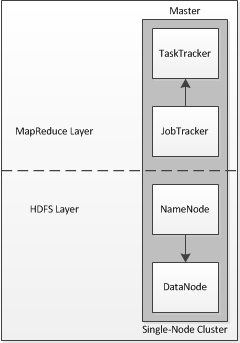
\includegraphics{./img/singlenode}
  \caption{Single-node Hadoop cluster \cite{nollsingle}.}
  \label{fig:singlenode}
\end{figure}

\subsection{Two-Node Cluster}
\cite{nollmulti}

\begin{figure}[htbp]
  \centering
    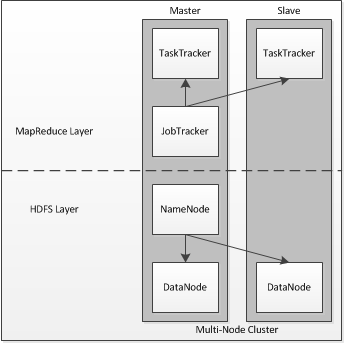
\includegraphics{./img/twonode}
  \caption{Two-nodes Hadoop cluster \cite{nollmulti}.}
  \label{fig:twonode}
\end{figure}

\subsection{Multi-Node Cluster}
At request, a nine machine Hadoop cluster was set up for use during this project in the department of computer science. This cluster composed a master head-node, {\tt hadoopmaster}, and eight slave-nodes, {\tt hadoop\{0-7\}}. 

Being the master, {\tt hadoopmaster} runs the NameNode, JobTracker and SecondaryNameNode processes. Each of the slave-nodes run the DataNode and TaskTracker processes.

HERE WILL BE SOME TECHNICAL SPECS ABOUT THE HADOOP CLUSTER IN THE DEPARTMENT

We did not have direct access to the Hadoop cluster, and were required to {\tt ssh} to a machine located within the department, before {\tt ssh}ing from this machine into the Hadoop cluster. This added an extra level of complexity to access the Hadoop cluster , yet was resolved though use of ssh-keys to allow this \emph{machine-in-the-middle} to send and receive files from hadoopmaster with requiring a password.